\subsection{Bifurcation Diagrams for Other Functions}
\begin{figure}[h!]
	\centering
	\begin{subfigure}{0.45\linewidth}
		\centering
		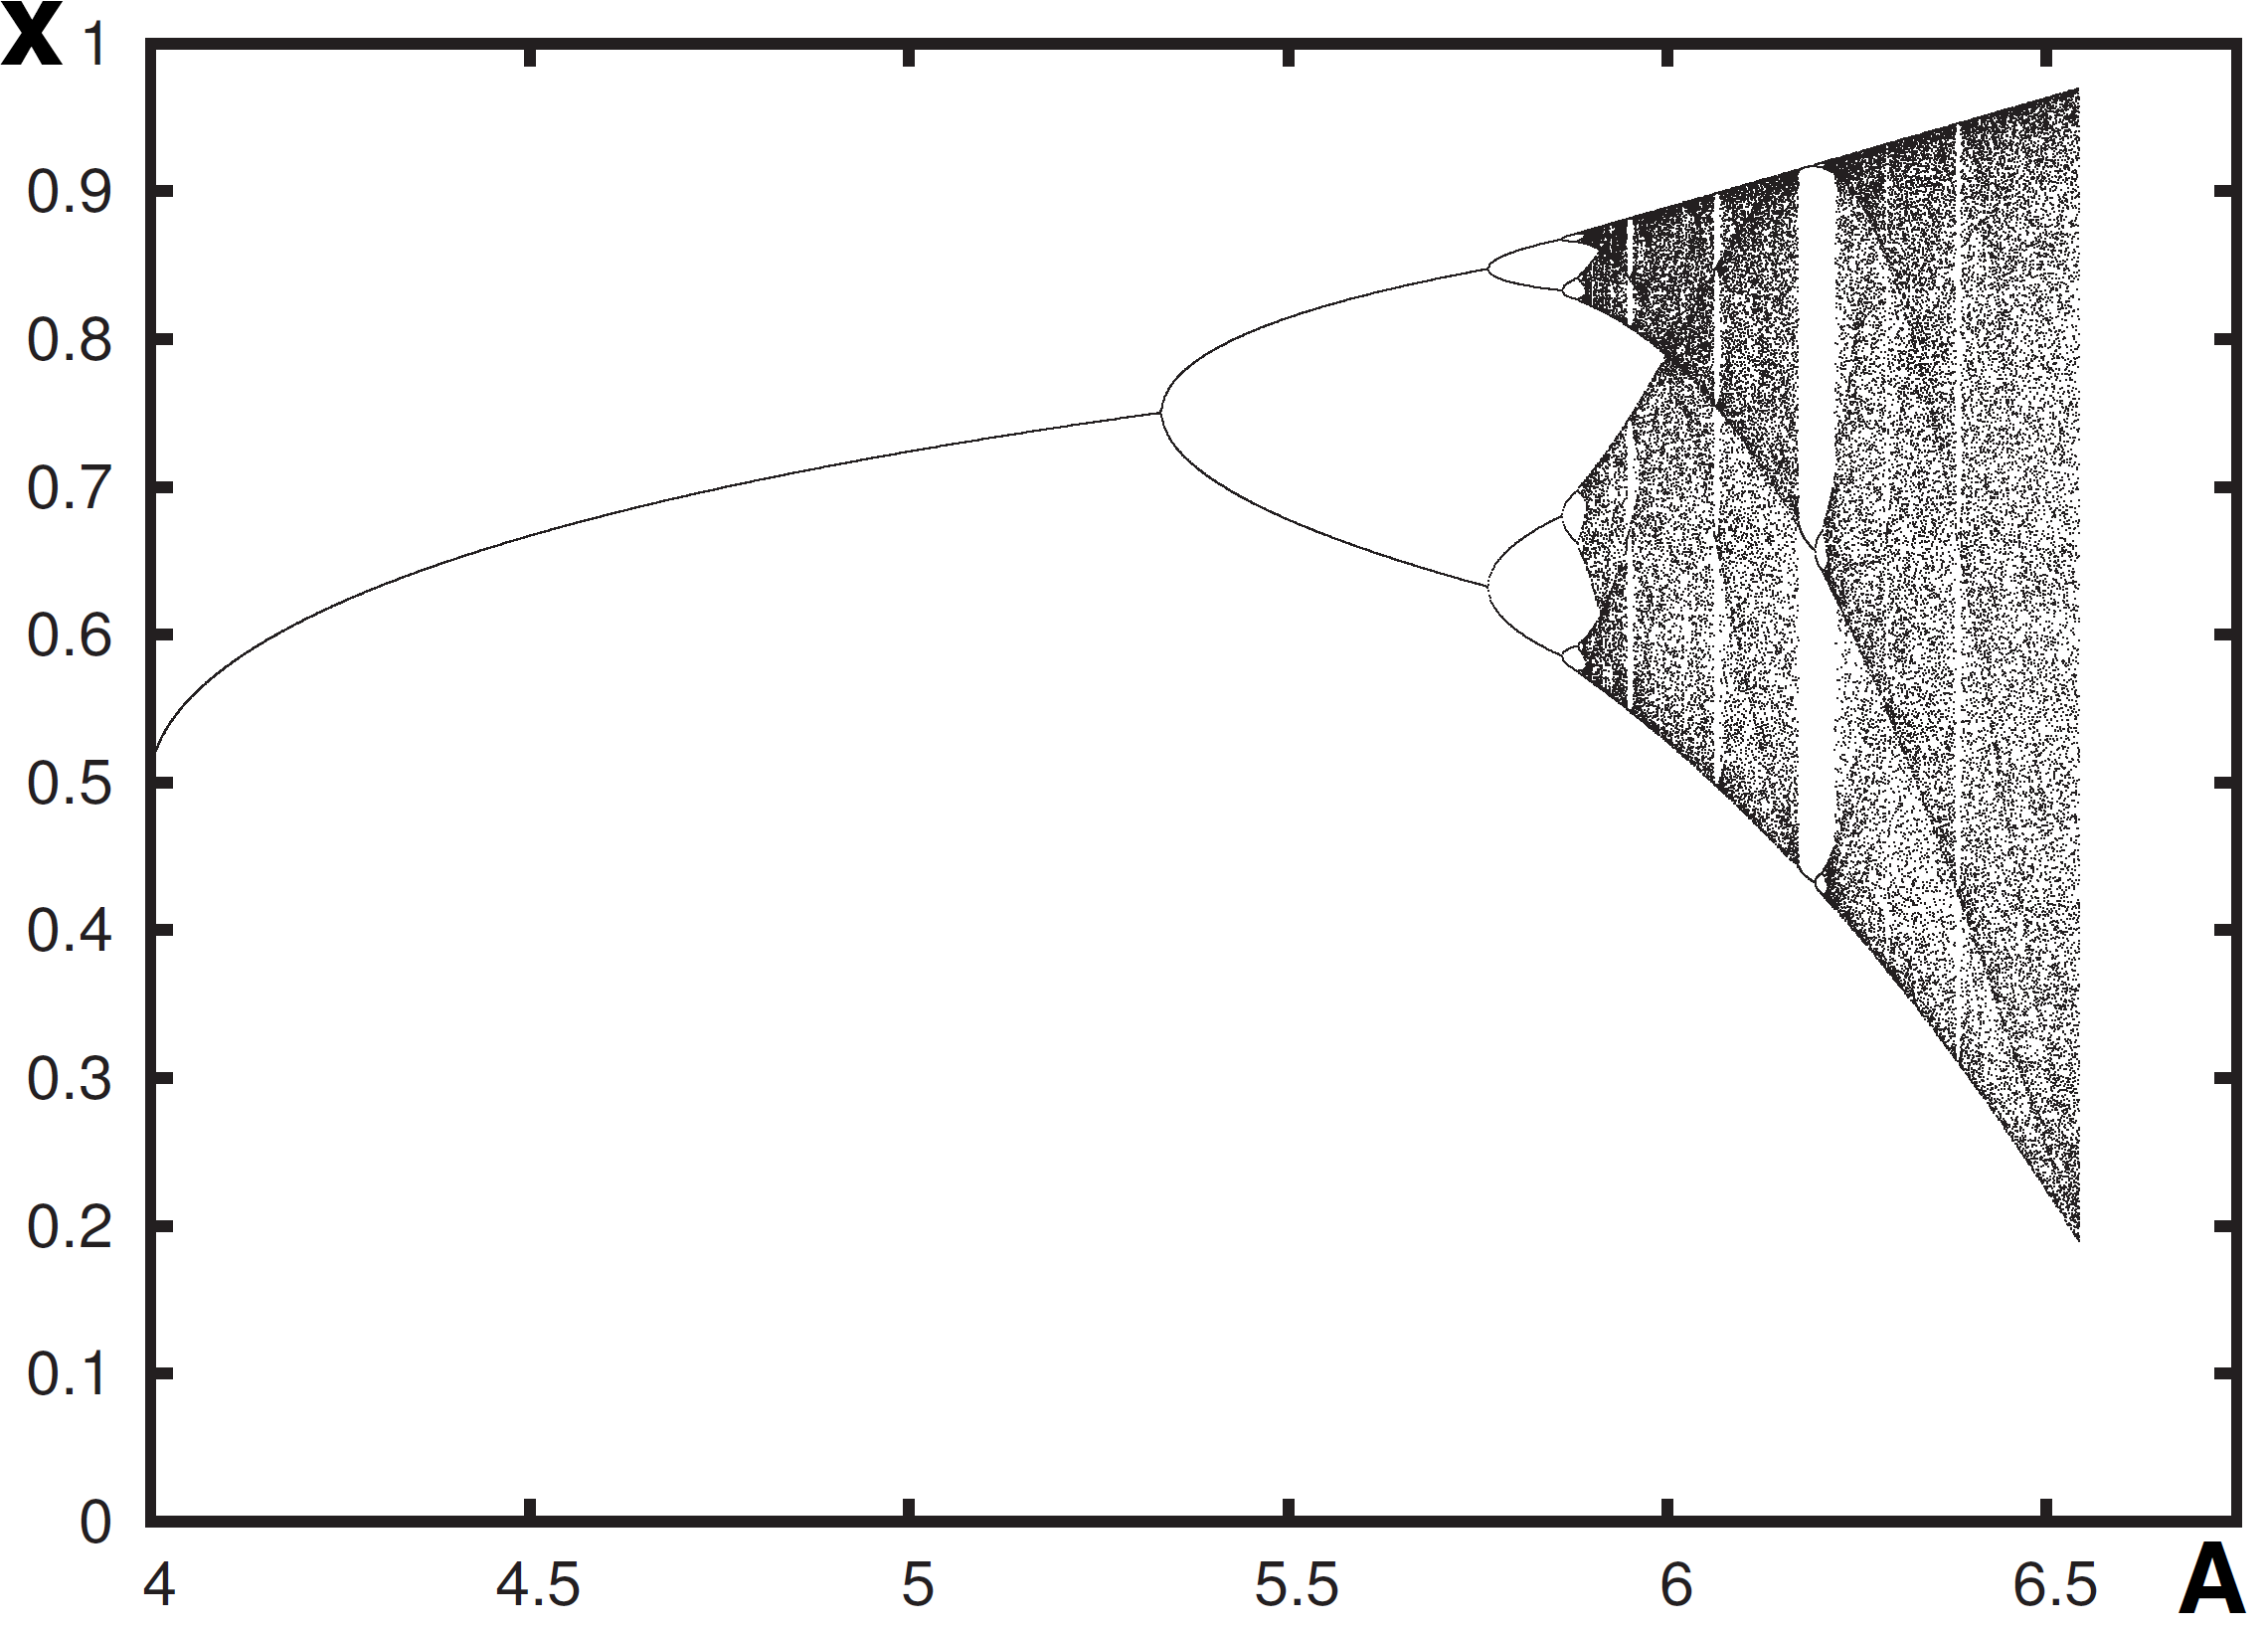
\includegraphics[width=\linewidth]{bfc.png}
		\caption{The bifurcation diagram for \\\centerline{$x_{n+1}=rx_n^2(1-x_n)$.}}
		\label{fig:bfc}
	\end{subfigure}
	\vline
	\begin{subfigure}{0.45\linewidth}
		\centering
		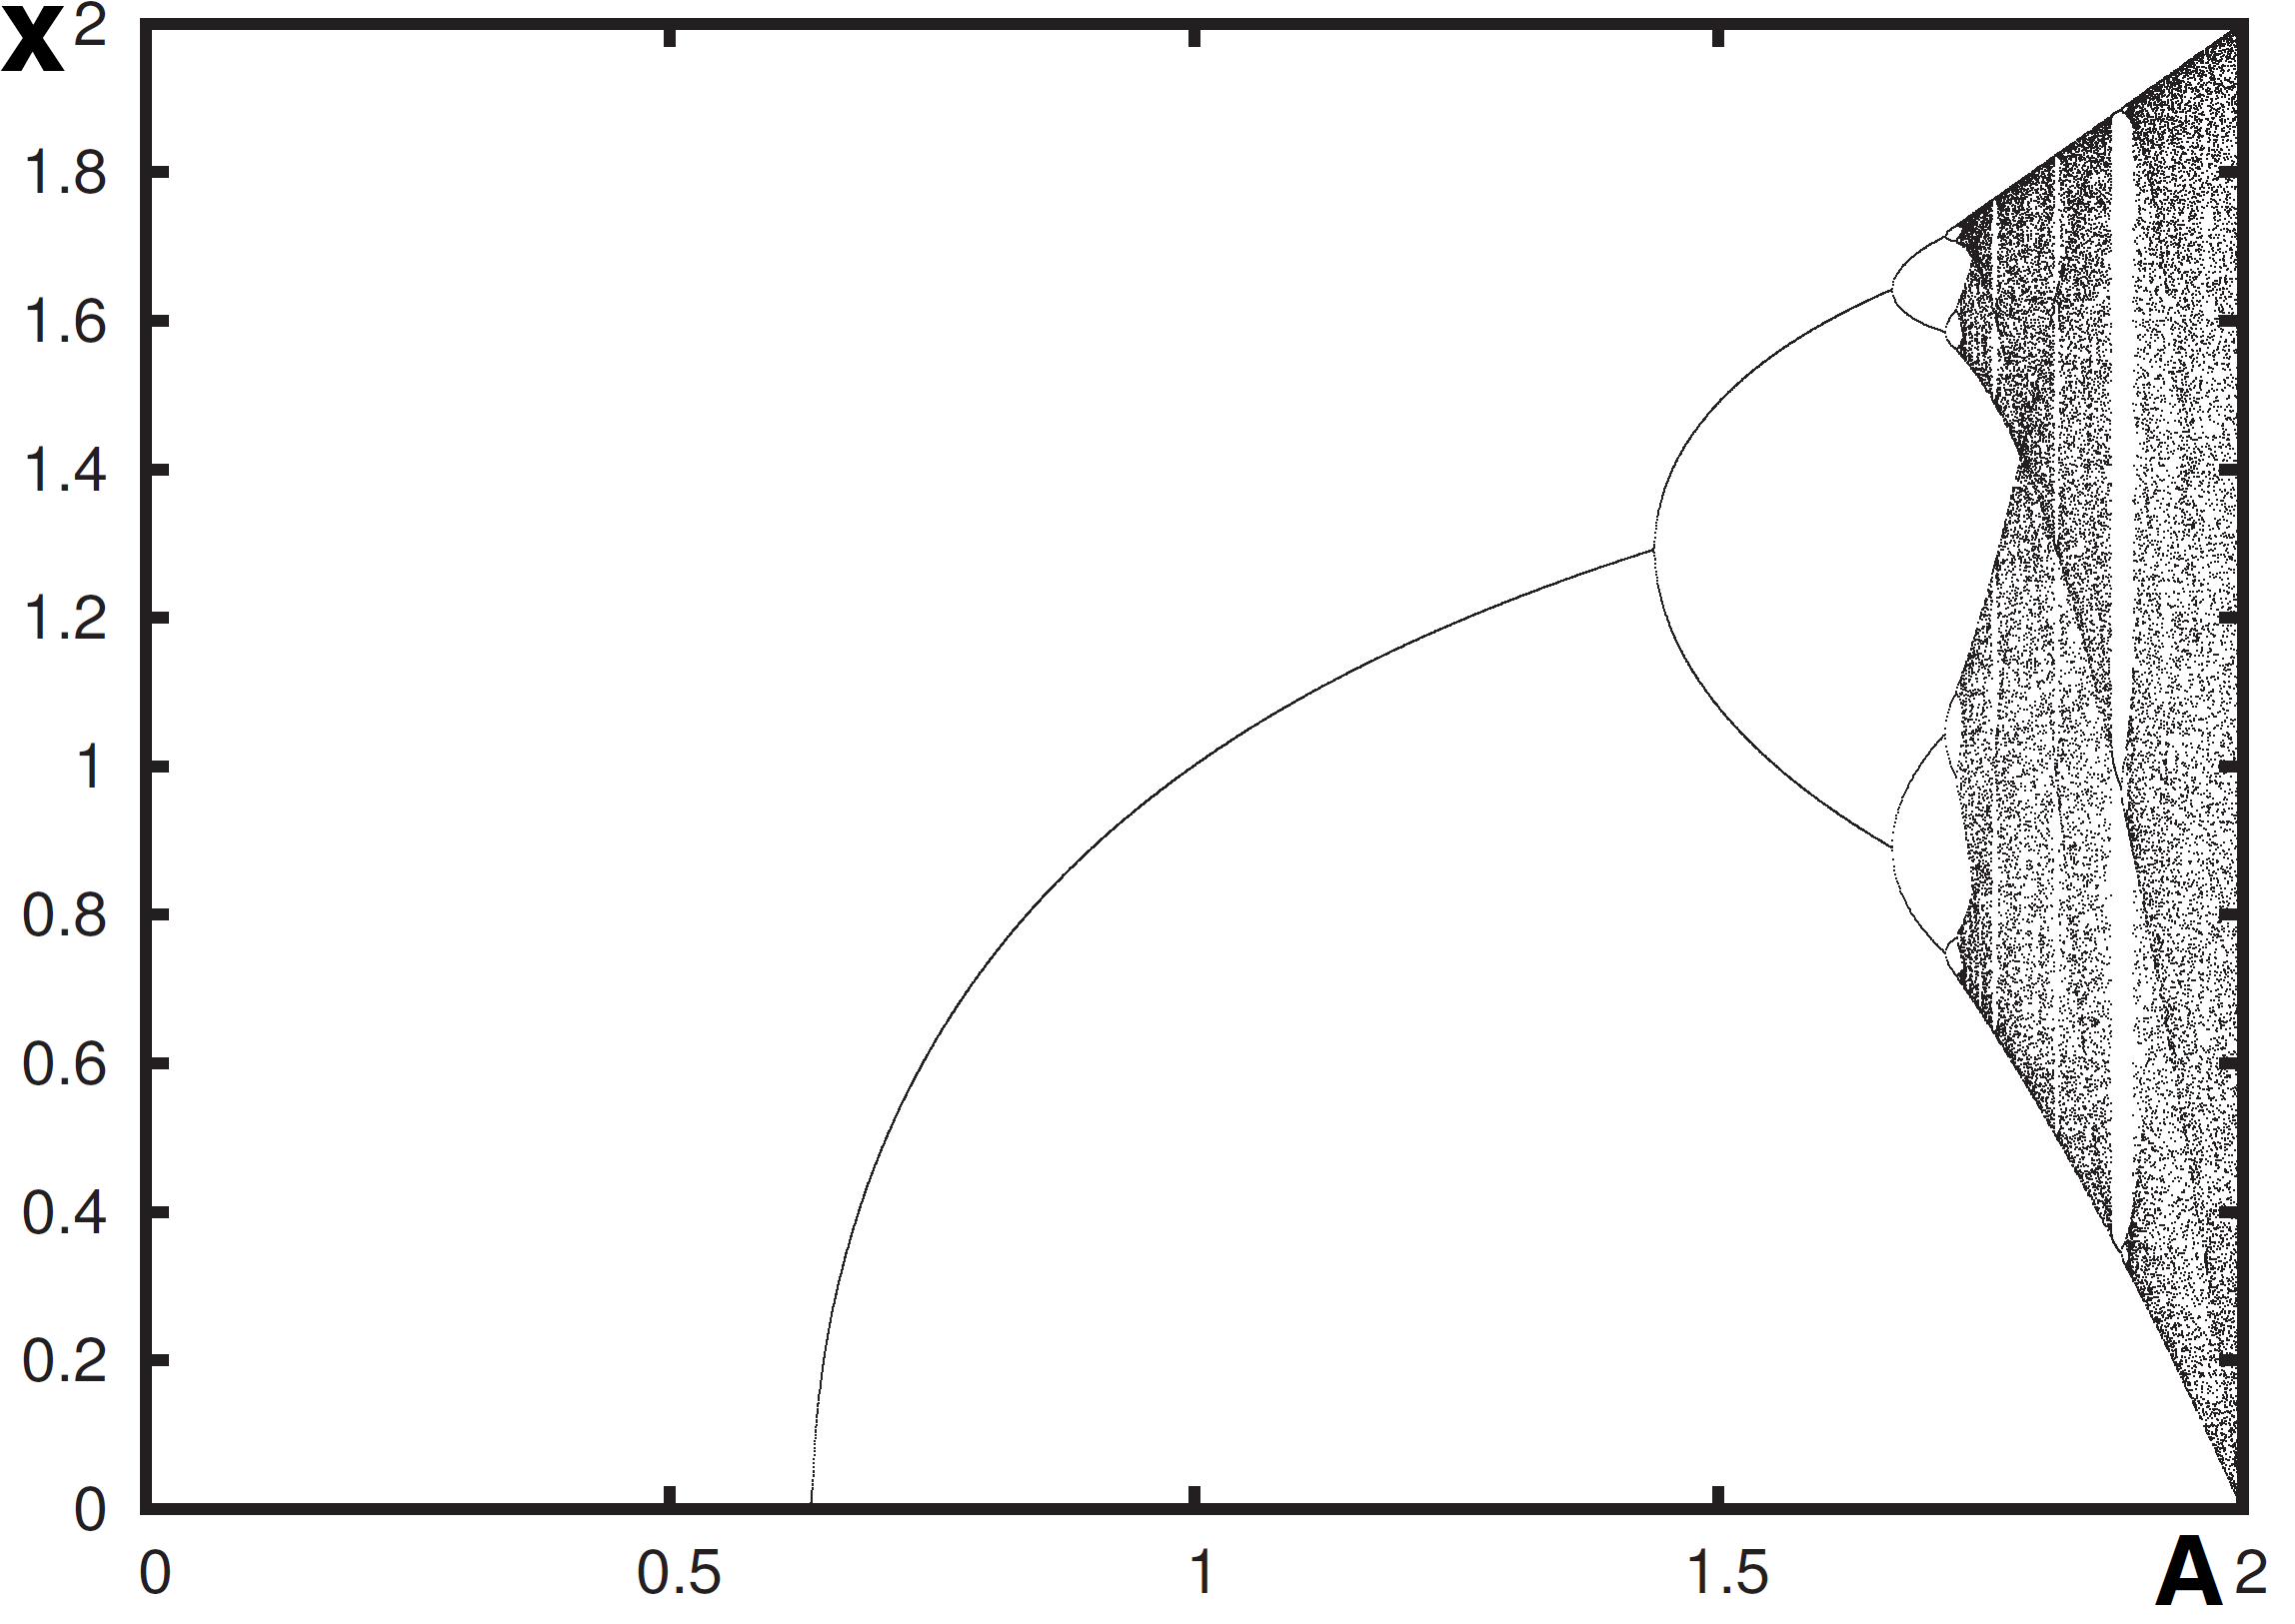
\includegraphics[width=\linewidth]{bfs.png}
		\caption{The bifurcation diagram for \\\centerline{$x_{n+1}=r\sin\left(\dfrac{\pi x_n}{2}\right)$.}}
		\label{fig:bfs}
	\end{subfigure}
	\caption{}
\end{figure}
Both systems given above has the \emph{same shape} as the graph of the logistic map.
Both curves are \emph{smooth}, \emph{concave} \emph{down}, and have a \emph{single} \emph{maximum}.
Such maps are called \textbf{unimodal}.
Both Bifurcations look similar.
In fact, we may at first think there has been some error and that logistic equation bifurcation diagram is accidentally used.
The \textbf{qualitative} dynamics of the two maps are identical.
They both undergo period-doubling routes to chaos, followed by periodic windows interwoven with chaotic bands.
\subsection{Qualitative Universality: U-Sequence}
The order in which stable periodic solutions appear is \emph{independent} of the unimodal map being iterated.
That is, the \emph{periodic} \emph{attractors} always occur in the \emph{same sequence}, now called the universal or \textbf{U-sequence}.
\subsection{Sharkovsky Ordering}
Consider the following ordering of natural numbers $a\prec b$ means $a$ comes before $b$
\begin{equation*}
	\begin{aligned}
		&1\prec2\prec2^2\prec2^3\prec\cdots\prec2^n\prec\cdots\prec7\cdot2^n\prec5\cdot2^n\prec3\cdot2^n\prec\cdots\prec7\cdot2\prec5\cdot2\prec3\cdot2\prec\cdots\prec7\prec5\prec3\\
		&\text{In general}\quad(1\prec2\prec2^2\prec\cdots\prec2^n\prec2^n\cdot k\prec\cdots\prec2^2\cdot k\prec2\cdot k\prec k)\quad\text{where $k$ are odd and decreasing}
	\end{aligned}
\end{equation*}
\begin{theorem}[\textbf{Sharkovsky Theorem}]
	If a continuous map of an interval into itself has a cycle of period $m$, then it has a cycle of any period $\tilde{m}\prec m$.
	Moreover, for any $m$ there exists a continuous map that has a cycle of period $m$ but does not have cycles of periods $\tilde{m},\ m\prec\tilde{m}$ .
\end{theorem}
The consequences of this amazing result are manifold:\\
If $f$ has a point of period 3, then $f$ has periodic points of any period.\\
If $f$ has a point of period $k\neq2^n$, then $f$ has infinitely many periodic points.